\begin{figure}[H]
    \center
    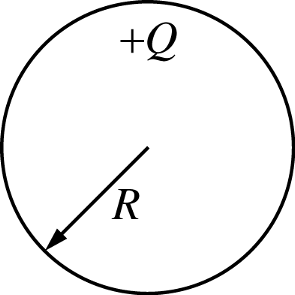
\includegraphics[scale=0.25]{images/img-010-020.png}
\end{figure}

% Multiple Choice Question 28
\begin{questions}\setcounter{question}{27}\question
The solid conducting sphere of radius $R$ shown above has a charge $+Q$ distributed uniformly on its surface. The potential at the center of the solid sphere is

\begin{oneparchoices}
\choice $+\dfrac{1}{4 \pi \epsilon_{0}} \dfrac{Q}{R}$
\choice $-\dfrac{1}{4 \pi \epsilon_{0}} \dfrac{Q}{R}$
\choice $-\dfrac{1}{4 \pi \epsilon_{0}} \dfrac{Q}{R^{2}}$
\choice Zero
\choice Undefined
\end{oneparchoices}\end{questions}

